\begin{figure}[h!]
    \centering
    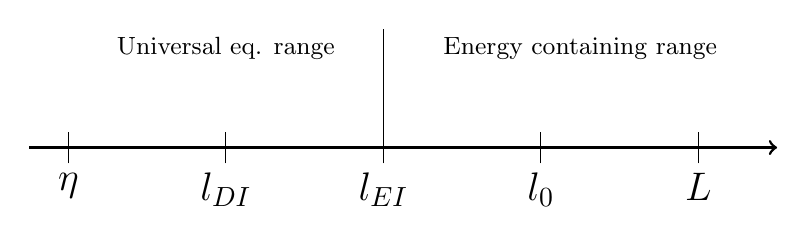
\begin{tikzpicture}
        \draw
            [->, black, line width = 1pt] (-5.5,0)--(4,0);
        \draw 
            (-5,-0.2) node[anchor=north]{\Large $\eta$}--(-5,0.2);
        \draw 
            (-3,-0.2) node[anchor=north]{\Large $l_{DI}$}--(-3,0.2);
        \draw 
            (-3, 1) node[anchor=south]{\small Universal eq. range};
        \draw 
            (-1,-0.2) node[anchor=north]{\Large $l_{EI}$}--(-1,0.2);
        \draw 
            (1,-0.2) node[anchor=north]{\Large $l_{0}$}--(1,0.2);
        \draw
            (-1,0.2)--(-1, 1.5);
        \draw 
            (1.5, 1) node[anchor=south]{\small Energy containing range};
        \draw 
            (3,-0.2) node[anchor=north]{\Large $L$}--(3,0.2);
    \end{tikzpicture}
    \caption{The different lengthscale's interplay in Kolmogorov's theory.}
    \label{fig:kolmogorov_scales}
\end{figure}